\chapter{Estado da Arte}
% OU \chapter{Trabalhos Relacionados}
% OU \chapter{Engenharia de Software}
% OU \chapter{Tecnologias e Ferramentas Utilizadas}
\label{chap:estado-da-arte}

\section{Introdução}
\label{chap2:sec:intro}

O reconhecimento e rastreamento de objetos é um dos campos mais atuais da visão computacional.
\newline É possivel reconhecer diferentes objetos em uma cena através das suas formas, cor e diferentes carateristicas do objeto.
É também possivel rastrear um objeto em um fluxo de video através do calculo de distâncias, comparação de formas, e outras carateristicas.
\newline Neste capitulo será abordado o estado atual do reconhecimento de objetos e o estado atual do rastreamento de objetos, e diferentes algoritmos que existem para o fazer. Isto com a especial atenção ao meio de desenvolvimento que será um Raspberry Pi, um pequeno computador com capacidades limitadas.
\paragraph{Este capítulo está estruturado da seguinte forma:}
\begin{enumerate}
  \item Secção 2.1 - \textbf{Estado atual do reconhecimento e rastreamento de objetos} - Esta secção apresenta uma introdução ao estado atual do reconhecimento e rastreamento de objetos, e uma explicação sobre algumas arquiteturas.
  \item Secção 2.2 - \textbf{Algoritmos de reconhecimento de objetos} - Esta secção apresenta vários algoritmos estudados sobre a deteção/reconhecimento de objetos e uma breve explicação do seu funcionamento. 
  \item Secção 2.3 - \textbf{Algoritmos de rastreamento de objetos} - Esta secção apresenta vários algoritmos estudados sobre o rastreamento de objetos, e uma breve explicação do seu funcionamento.
  \item Secção 2.4 - \textbf{Conclusões} - Esta secção apresentará uma breve conclusão sobre este capitulo.
\end{enumerate}


\section{Estado atual do reconhecimento e rastreamento de objetos}
\label{chap2:sec:estadoatual}

Para entendermos o estado atual do reconhecimento de objetos, é preciso ver uma breve história do reconhecimento de objetos até ao estado atual e entender algumas definições.

\paragraph{}
A deteção de objetos combina as tarefas de localização e classificação de objetos. Os detetores de objetos atuais podem ser divididos em duas categorias:
\newline - Redes que separam as tarefas de determinar a localização dos objetos e sua classificação, onde \texttt{Faster \ac{R-CNN}} é uma das mais famosas.
\newline - Redes que prevêm caixas delimitadoras e classificações de classes de uma só vez, onde as redes \texttt{\ac{YOLO}} e \texttt{\ac{SSD}} são famosas arquiteturas.

\paragraph{}
A primeira rede neural profunda para deteção de objetos foi \texttt{Overfeat}. Eles introduziram uma abordagem de janela deslizante de várias escalas usando \texttt{\ac{CNN}} e mostraram que a deteção de objetos também melhorou a classificação de imagens.
Foram logo seguindos por \texttt{\ac{R-CNN}}: Regiões com carateristicas \texttt{\ac{CNN}}. Os autores proposerão um modelo que usa pesquisa seletiva (selective-search) para gerar as proporções da região, mesclando pixels semelhantes em regiões. Cada região foi alimentada em uma \texttt{\ac{CNN}}, que produziu um vetor de carateristica de grande dimenção. Este vetor é depois usado para a classificação final e regressão da caixa delimitadora, como mostra na figura \ref{img:rcnn}.


\begin{figure}[h!]
  \label{img:rcnn}
  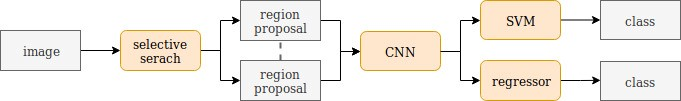
\includegraphics[width=1\textwidth]{rcnn.jpeg}
  \caption{A arquitetura padrão de uma rede \ac{R-CNN} consiste em um metodo de proporção regional. A classificação final é feita com uma \ac{SVM} e um regressor.}
\end{figure}


\paragraph{}
\ac{SVM} é um conjunto de métodos de aprendizado supervizionado que analizam os dados e reconhecem padrões, usando classificação e análise de regressão.

\paragraph{}
Uma abordagem mais sotisficada, o \texttt{Fast \ac{R-CNN}} também gera proporções regionais com pesquisa selectiva, mas alimenta a imagem inteira através de uma \texttt{\ac{CNN}}.
Ela superou o desempenho da rede \texttt{Overfeat} por uma grande margem, mas ainda assim é muito lenta, porque a geração proposicional usando pesquisa seletiva é muito demorada, tal como a necessidade de alimentar cada proposta através de uma \texttt{\ac{CNN}}. As proporções regionais são agrupadas diretamente em um mapa carateristico por \texttt{\ac{ROI} pooling}. Os vetores carateristicos agrupados são alimentados em uma rede totalmente conectada para classificação e regressão, como retratado na figura \ref{img:fastrcnn}. Similar ao \texttt{\ac{R-CNN}}, o \texttt{Fast \ac{R-CNN}} gera as proporções regionais usando pesquisa seletiva.

\paragraph{}
\texttt{\ac{ROI} pooling}, ou agrupemento da Região de Interesse é o processo de converter uma região de interesse da imagem original em uma imagem de tamanho fixo para que se possa passar à proxima etapa de deteção do objeto.

\begin{figure}[h!]
  \label{img:fastrcnn}
  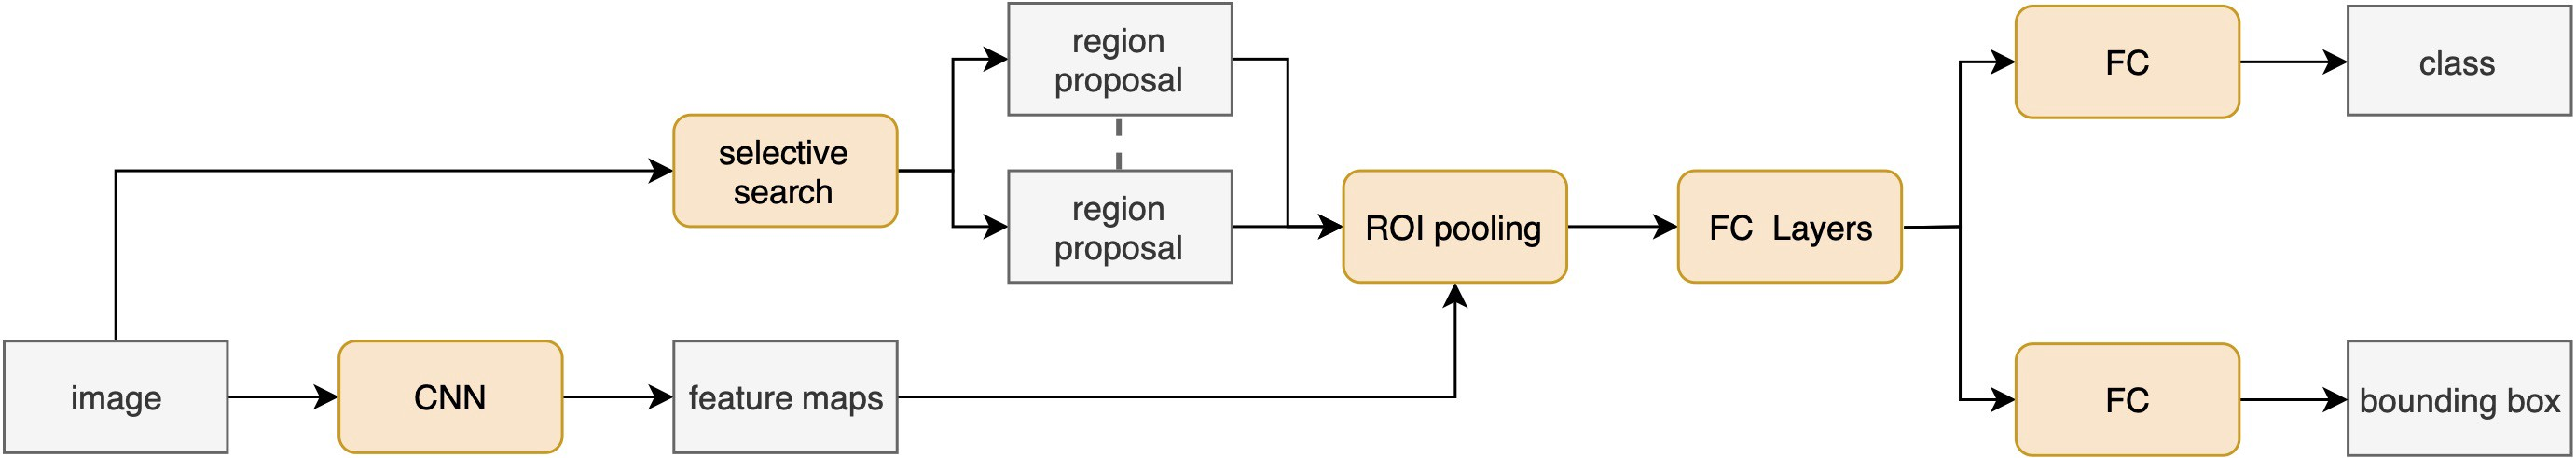
\includegraphics[width=1\textwidth]{fastrcnn.jpeg}
  \caption{A arquitetura padrão da rede \texttt{Fast-\ac{R-CNN}}. A proporção regional é gerada usando pequisa seletiva, mas agrupada diretamente no mapa de carateristicas, seguida de várias camadas \texttt{FC} para a classificação final e regressão da caixa delimitadora.}
\end{figure}

\paragraph{}
\texttt{Faster \ac{R-CNN}} abordou esta questão propondo uma nova rede de proporção regional, que foi unida com a arquitetura \texttt{Fast \ac{R-CNN}} para drasticamente aumentar a velocidade do processo. Outra abordagem para a deteção de objetos em imagens é o \texttt{\ac{R-FCN}}, uma rede totalmente convolucional da região, que usa mapas de pontuação sensiveis à posição em vez de uma sub-rede pré-região.

O design das redes de deteção de objetos foi revolucionado pela rede \texttt{\ac{YOLO}}. Este segue uma abordagem completamente diferente dos modelos mencionados e é capaz de prever classificações de classes e caixas delimitadoras de uma vez. O modelo proposto divide a imagem em uma grelha, onde cada celula preve classificações de confiança de um objeto estar presente com as coordenadas da caixa delimitadora correspondente. Isto permitiu previsões em tempo real com o \texttt{\ac{YOLO}}. Os autores libertaram mais três versões, YOLO9000, YOLOv2 e YOLOv3, onde o primeiro é capaz de prever até 9000 categorias, o segundo é capaz de processar imagens maiores e o terceiro é mais preciso. Outra rede que preve classes e caixas delimitadoras de uma vez é o \texttt{\ac{SSD}}. É comparavel com o \texttt{\ac{YOLO}}, mas usa várias proporções por célula da grelha e mais camadas convolucionais para melhorar a precisão.


\begin{figure}[h!]
  \label{img:fasterrcnn}
  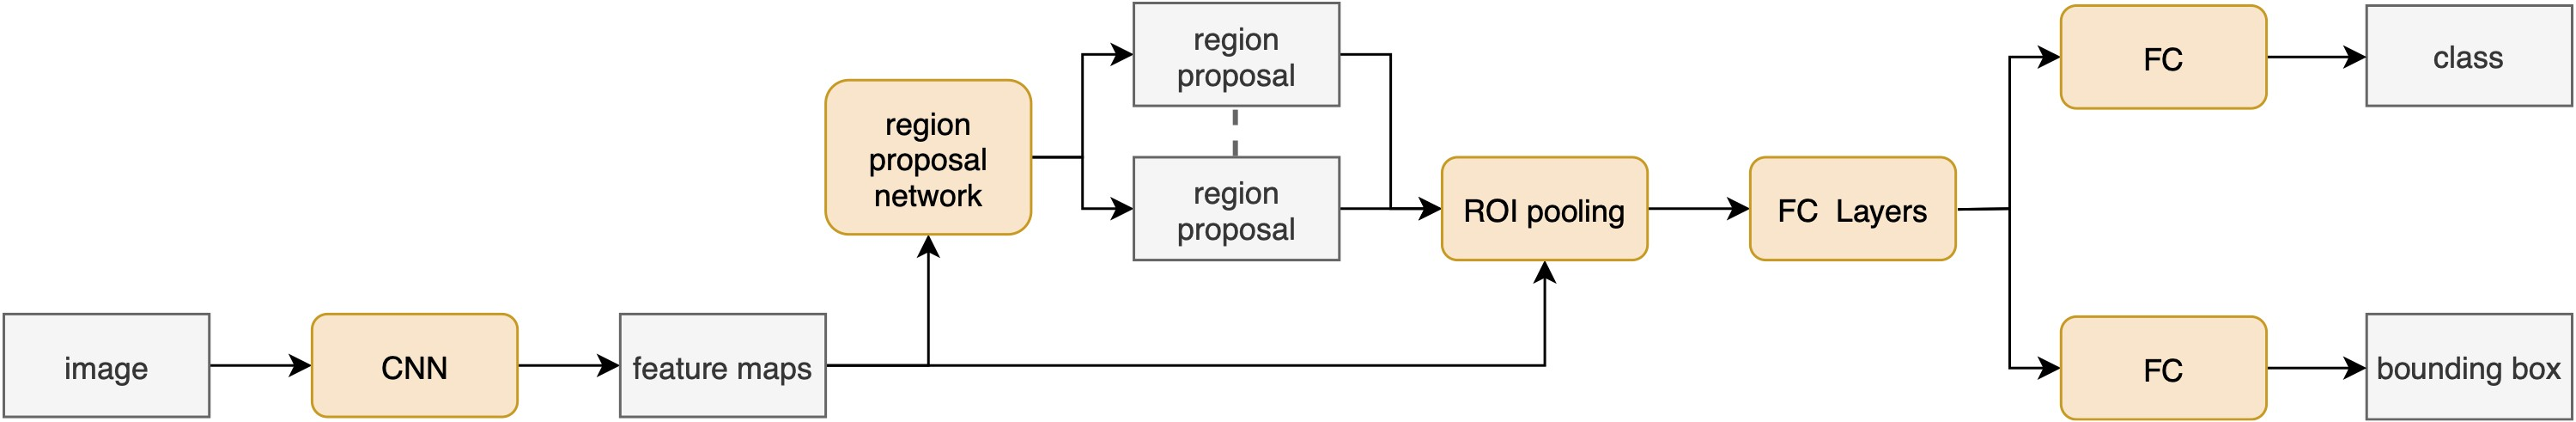
\includegraphics[width=1\textwidth]{fasterrcnn.jpeg}
  \caption{A arquitetura padrão da rede \texttt{Faster-\ac{R-CNN}}, onde a proposta de região é gerada usando uma RPN, que trabalha diretamente com o mapa de carateristicas. As ultimas camadas estão totalmente connectadas para classificação e regressão das caixas delimitadoras.}
\end{figure}


https://towardsdatascience.com/understanding-object-detection-9ba089154df8


\section{Algortimos de Deteção de Objetos}
\label{chap2:subsec:algoritmosdetecao}

\subsection{Haar cascades}

Este método foi proposto por P. Viola e M. Jones em 2001. EM resumo, é um método de aprendizagem de máquina (Machina Learning) onde uma função chamada cascata é treinada em uma grande quantidade de imagens positivas e negativas (positivas significam que contêm o objeto especificado e negativas que não contem), que por sua vez podem ser usadas para a deteção de objetos.

Para isto vou explicar o conceito dos recursos Haar, estes são obtidas pelas caixas a preto e branco abaixo que atuam como Kernels convolucionais. Os recursos são mais expecificamente valores unicos recebidos através da subtração da soma dos pixels dos retangulos brancos da soma dos pixels dos retangulos pretos.


imagem 1


Se estiver desconfortável com a palavra convolução, esta é essencialmente o resultado de duas funções afetando uma à outra. Portanto, no nosso caso, isto significa, como a soma dos pixels na parte das caixas a preto e branco interagem, ou seja, são diferenciados para produzir um unico valor. Já existe um algoritmo para calcular a soma dos pixels eficientemente dentro de uma area, é chamado tabela de àrea resumida e foi publicado por F. Crow em 1984. Este foi posteriormente popularizado no dominio do processamento de imagens e fica sobre o nome de imagem integral.


imagem 2

Tentamos diferentes recursos Haar e vemos qual produz o maior valor para a diferença entre a soma dos pixels entre os retangulos pretos e brancos. Temos abaixo um exemplo onde recursos Haar otimizados foram encontrados. Os olhos são normalmente um pouco mais escuros, onde a area abaixo é provavelmente mais clara, e assim um retangulo horizontal com preto no topo e branco em baixo é adequado. Em segundo lugar a ponte do nariz geralmente é mais clara que os olhos e então, um recurso de Haar com uma caixa branca vertical no meio é mais adequada.


imagem 3

....


https://towardsdatascience.com/object-detection-with-haar-cascades-in-python-ad9e70ed50aa



\subsection{HOG + Linear SVM}
Neste algortimo, conhecido como Single Shot Detector (Detector de com apenas uma foto), tiramos apenas uma foto para detetar multiplos objetos presentes em uma unica imagem usando multibox (multiplas caixas).
É significamente mais rápido em velocidade e grande precisão em algoritmos de deteção de objetos.
\newline
A rápida velocidade e precisão do SSD usando relativamente imagens com baixa resolução é atribuida devido às seguintes razões:
\newline - Remove caixas delimitadoras como as que são usadas em R-CNN's
\newline - Inclui um filtro convulucional progressivamente decrescente para prever as categorias dos objetos e compensações no lugar das caixas delimitadoras.
\newline
A Alta presição de deteção no SSD é obtida usando multiplas caixas ou filtros com diferentes tamanhos, e proporção de tela para a deteção de objetos. Isto também aplica esses filtros a vários mapas de recursos dos estágios posteriores de uma rede. Isso ajuda a executar a deteção em várias escalas.

\subsection{SSDs}

\subsection{Faster R-CNNs}

\subsection{Yolo}
\paragraph{}
\textit{\ac{Yolo} (You Only Look Once)} é um algortimo de deteção de objetos que aceita um feed de video em tempo real.
No Yolo, com uma unica CNN ??? ??? simultanemente prevemos multiplas caixas delimitadoras e probabilidades de classes para essa caixa. O Yolo treina em imagens completas e otimiza diretamente o desempenho da deteção. Este modelo afirma ter um numero de beneficios sobre outros métodos de deteção de objetos, como:
\newline - YOLO encontra todos os objetos em uma imagem simultanemente.
\newline - Usa uma unica rede convulcional para toda a imagem.
\newline - Usa carateristicas da imagem inteira para prever cada caixa.delimitadora. Tambem preve todas as caixas delimitadoras de todas as classes para uma imagem simultanemanete. Prevê as caixas delimitadoras e as probabilidades de classe para essas caixas.
\newline - YOLO vê a imagem inteira durante o treino e tempo de teste, portanto codifica implicitamente informações contextuais sobre classes tal como a sua aparencia.
\newline - YOLO aprende representações generalizadas de objetos para que quando treinado em imagens naturais e testado em obras de arte, o algoritmo supera outros modelos de deteção.

\paragraph{Trabalho do YOLO}
\paragraph{}

- YOLO pega em uma imagem e divide-a em uma rede SxS. Cada célula prevê apenas um objeto.
- A clissificação e localização da imagem são aplicados em cada célula.
- Se o centro de um objeto fica em uma célula, essa célula é responsavel por detetar esse objeto.
- Cada célula da rede prevê B caixas delimitadoras com classificações de confiança para essas caixas.

1. Caixas de confiança refletem o quão confiante o modelo está sobre a caixa conter o objeto e quão preciso ele pensa a caixa ser o que ele pensa. Se o objeto não existir, então a classificação de confiança será zero. 
\newline
A previsão de confiança reprensenta a IOU entre a caixa de previsão e qualquer caixa de verdade do solo.
Pr(Object) * IOU verdade previsão - interseção de união (\ac{IoU}) entre a caixa prevista e o verdadeiro solo.







The output of the algorithm is a list of bounding box, in format [class, x, y, w, h, confidence]. The class is an id related to a number in a txt file (0 for car , 1 for pedestrian, …). x, y, w and h represent the parameters of the bounding box. x and y are the coordinates of the center while w and h are its size (width and height). The confidence is a number expressed in %.

\subsection{Tensorflow}
\label{chap2:subsec:tensorflow}

Tensorflow Lite


\subsection{OpenCV}
\label{chap2:subsec:opencv}
\paragraph{}

Opencv é uma biblioteca \textit{open source} criada em 2000 pela Intel e com Licença BSD Intel para a sua Distribuição. Utilizada para o desenvolvimento de aplicações na área de computação visual, seja para o uso acadêmico ou comercial. Possui módulos para processamento de imagens, estrutura de dados, àlgebra linear, bem como uma interface gráfica para usuário e mais de 350 algoritmos de visão computacional, como filtros de imagem, calibração de câmera, reconhecimento de objetos, análise estrutural e outros.


\section{Algortimos de Rastreamento de Objetos}
\label{chap2:subsec:algoritmosrastreamento}



\subsection{Centroid tracking}
\label{chap2:subsec:centroidtraking}



\paragraph{}
\textit{Centroid traking} é um algoritmo presente na biblioteca OpenCV, que depende da distância euclidiana\footnote{Dintância entre dois pontos} entre centróides de objetos (ex. objetos que o rastreador de centróide já viu antes) e novos centróides de objetos entre quadros subsequentes em um video.

O algoritmo de rastreamento de centróides é um processo de multiplas etapas:

\paragraph{1- Aceitar as coordenadas da caixa delimitadora do objeto e calcular os centróides}
\paragraph{}
Este algoritmo assume que estamos a passar um conjunto delimitador de coordenadas 2D de cada objeto detectado em \textit{every single frame} (cada frame de video).
\newline
Estas caixas delimitadoras podem ser produzidas por qualquer tipo de detetor de objetos que mais gostemos (temos em este capitulo alguns algoritmos de delimitadores explicados).
\newline
Depois de obtermos as coordenadas das caixas delimitadoras, devemos determinar o centróide, ou simplesmente, o centro da caixa.
\newline
Visto que este é o conjunto inicial de caixas, devemos lhes atribuir IDs unicos.
\begin{center}
  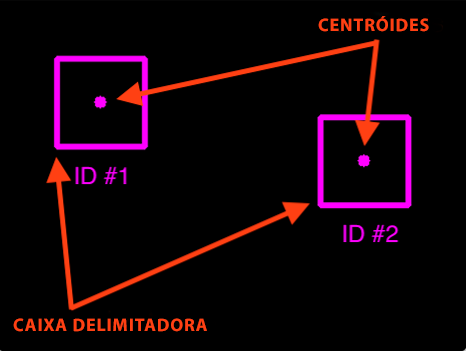
\includegraphics[scale=0.5]{simple_object_tracking_step1.png}
  \label{img:centroid_traking1}  
\end{center}

\paragraph{2- Calcular distância euclediana entre novas caixas delimitadoras e objetos existentes}
\paragraph{}
Para cada subsequente frame do nosso video, aplicamos a etapa 1 de calcular os centróides de cada objeto. Porem aqui, invês de atribuir um ID unico a cada objeto detectado (que iria contrariar o sentido de rastrear um objeto), precisamos determinar primeiro se podemos acociar novos centróides de objetos (pontos amarelos) a aos centróides antigos (pontos roxos). Para este processo, nós calculamos a distância euclediana entre cada par de objetos existente e novos objetos.
\newline
Mas como vamos usar as distâncias Eucledianas entre estes pontos para combiná-los e associá-los? 

\begin{center}
  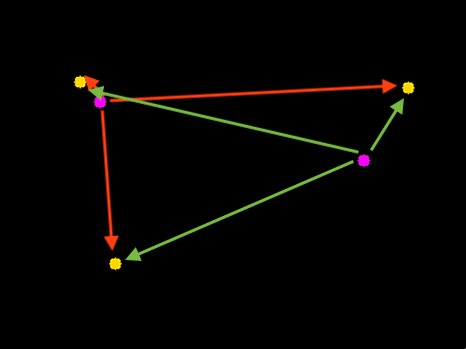
\includegraphics[scale=0.5]{simple_object_tracking_step2.png}
  \label{img:centroid_traking2}  
\end{center}

\paragraph{3- Atualizar coordenadas para objetos existentes}
\paragraph{}
A supozição primária do algoritmo de rastreamento de centroides de objetos é de que o objeto irá se potencialemente mover entre frames subsequentes, porem a distância entre centróides será menor que outras distâncias entre objetos.
\newline
Portanto, se escolhermos associar centróides com a menor distância entre frames subsequentes, podes construir o nosso rastreador de objetos.
\newline
Mas e se surgir um novo objeto? 

\begin{center}
  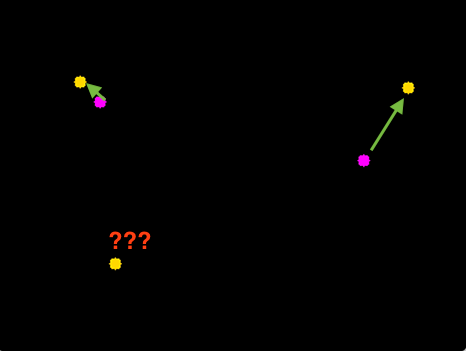
\includegraphics[scale=0.5]{simple_object_tracking_step3.png}
  \label{img:centroid_traking3}  
\end{center}


\paragraph{4- Registar novos objetos}
\paragraph{}
No caso de obtermos mais objetos detetados do que objetos a ser rastreados, precisamos registar o novo objeto. Registar o novo objeto na lista de objetos a ser rastreados significa que: 
\newline - Atribuimos um novo ID
\newline - Guardamos o centróide da caixa delimitadora para esse objeto
\newline
Podemos ir até a etapa 2 e repetir o processo de etapas em cada frame de video.

\begin{center}
  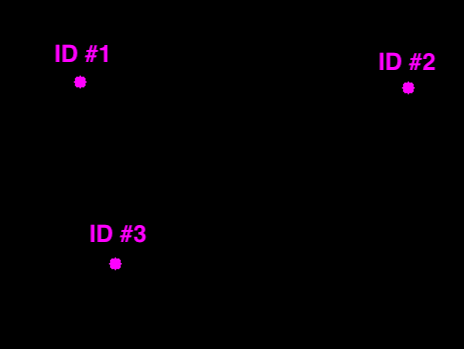
\includegraphics[scale=0.5]{simple_object_tracking_step4.png}
  \label{img:centroid_traking4}  
\end{center}



ref: 
https://www.pyimagesearch.com/2018/07/23/simple-object-tracking-with-opencv/


\subsection{Hungarian Algorithm (Kuhn-Munkres)}
\label{chap2:subsec:hungarian}

A Hungarian algorithm can tell if an object in current frame is the same as the one in previous frame. It will be used for association and id attribution

https://towardsdatascience.com/computer-vision-for-tracking-8220759eee85

\subsection{Kalman Filter}
\label{chap2:subsec:kalman}


A Kalman Filter is an algorithm that can predict future positions based on current position. It can also estimate current position better than what the sensor is telling us. It will be used to have better association.

https://towardsdatascience.com/computer-vision-for-tracking-8220759eee85




































\section{Citações e Referências Cruzadas -- [RETIRAR DA VERSÃO FINAL]}
\label{chap2:sec:citacoes}

Para se referenciarem outras secções, usar \texttt{\textbackslash{}ref\{label\}}, e.g., para citar a secção da Introdução deste capítulo, usar \texttt{\textbackslash{}ref\{chap2:sec:intro\}}. O resultado é: a secção~\ref{chap2:sec:intro} contém a introdução deste capítulo.

Para se citarem fontes bibliográficas, \underline{colocar a entrada certa} no ficheiro \texttt{bibiografia.bib} e usar o comando \texttt{\textbackslash{}cite\{label-da-referencia\}}, ligando o comando com a palavra que o antecede com um til. Por exemplo, para citar a referência eletrónica \emph{The Not So Short Introduction to \LaTeX{}}~\cite{short}, deve incluir-se o trecho seguinte no ficheiro \texttt{bibiografia.bib} e usar \texttt{\textbackslash{}cite\{\underline{short}\}} para a citação (citação incluída nesta mesma frase):
%
\begin{verbatim}
@MISC{short,
  author = {Tobias Oetiker and Hubert Partl and Irene Hyna and Elisabeth Schlegl},
  title  = "{The Not So Short Introduction to \LaTeX{}}",
  year   = 2018,
  note   = {[Online] \url{https://tobi.oetiker.ch/lshort/lshort.pdf}. 
            Último acesso a 12 de Março de 2019}
}
\end{verbatim}


\section{Secções Intermédias}
\label{chap2:sec:...}

\section{Conclusões}
\label{chap2:sec:concs}

Cada capítulo \underline{intermédio} deve referir o que demais importante se conclui desta parte do trabalho, de modo a fornecer a motivação para o capítulo ou passos seguintes.